\documentclass[tikz,border=10pt]{standalone}
\usepackage[T1]{fontenc}
\usepackage[utf8]{inputenc}
\usepackage{tikz}
\usetikzlibrary{arrows.meta, positioning, fit}

\begin{document}
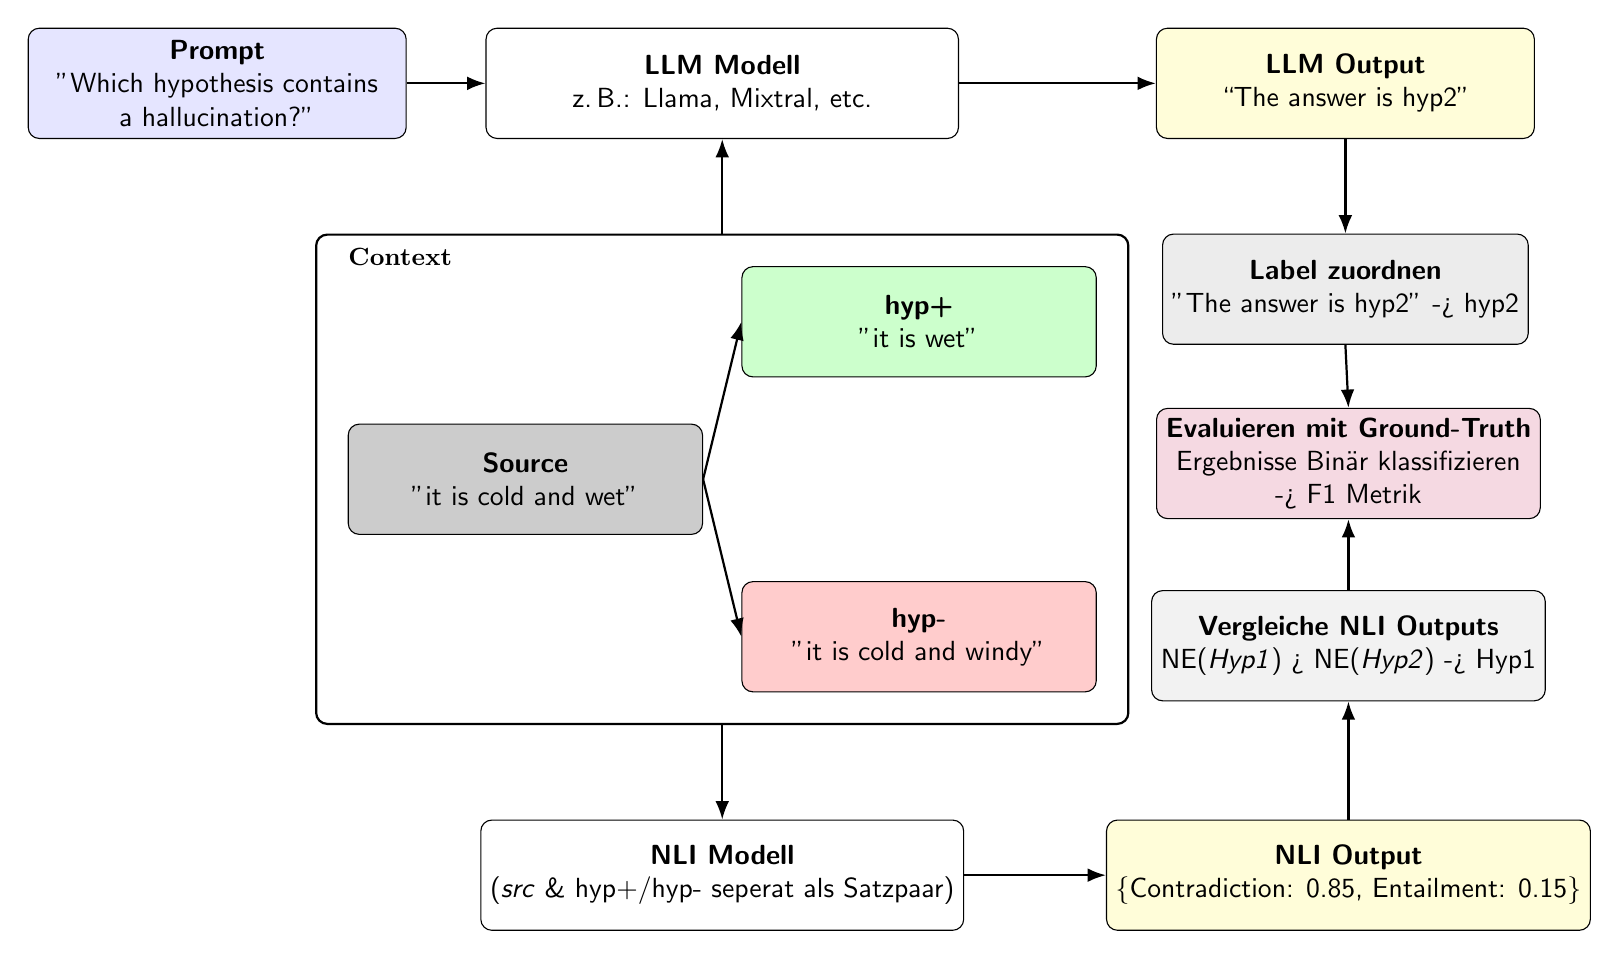
\begin{tikzpicture}[
  font=\sffamily,
  box/.style={
    draw,
    rounded corners,
    align=center,
    minimum width=4.5cm,
    minimum height=1.4cm
  },
  arrow/.style={-Latex, thick}
]

% --- Context content ---
\node[box, fill=black!20] (src) {\textbf{Source}\\ "it is cold and wet"};

\node[box, xshift=50mm, yshift=20mm, fill=green!20] (hyp1)
{\textbf{hyp+}\\ "it is wet"};

\node[box, xshift=50mm, yshift=-20mm, fill=red!20] (hyp2)
{\textbf{hyp-}\\ "it is cold and windy"};

\draw[arrow] (src.east) -- (hyp1.west);
\draw[arrow] (src.east) -- (hyp2.west);

% --- Context frame ---
\node[
  draw,
  rounded corners,
  thick,
  fit=(src)(hyp1)(hyp2),
  inner sep=4mm
] (context) {};

% Context label
\node[anchor=west, font=\small]
at ([xshift=3mm,yshift=-3mm]context.north west)
{\textbf{Context}};

% --- Model ---
\node[box, above=12mm of context, minimum width=6cm] (model)
{\textbf{LLM Modell}\\ z.\,B.: Llama, Mixtral, etc.};

\draw[arrow] (context.north) -- (model.south);

% --- Prompt (left into model) ---
\node[box, left=10mm of model, fill=blue!10, minimum width=4.8cm] (prompt)
{\textbf{Prompt}\\
"Which hypothesis contains\\ a hallucination?"};

\draw[arrow] (prompt.east) -- (model.west);

% --- Output (right from model) ---
\node[box, right=25mm of model, fill=yellow!15, minimum width=4.8cm] (output)
{\textbf{LLM Output}\\
“The answer is hyp2"};

\node[box, below=12mm of output, fill=gray!15, minimum width=4cm](llmeval)
{\textbf{Label zuordnen} \\ "The answer is hyp2" -> hyp2};


\draw[arrow] (output.south) -- (llmeval.north);

\node[box, below=12mm of context, minimum width=4.8cm] (NLI) 
{\textbf{NLI Modell} \\(\textit{src} \& hyp+/hyp- seperat als Satzpaar)};

\node[box, right=18mm of NLI, fill=yellow!15, minimum width=4.8cm](nlioutput) {\textbf{NLI Output} \\ \{Contradiction: 0.85, Entailment: 0.15\}};

\draw[arrow] (NLI.east) -- (nlioutput.west);



\node[box, above=15mm of nlioutput, fill=gray!10, minimum width=4.8cm] (nlinorm)
{\textbf{Vergleiche NLI Outputs} \\ NE(\textit{Hyp1}) > NE(\textit{Hyp2}) -> Hyp1};

\node[box, above=9mm of nlinorm, fill=purple!15, minimum width=4.8cm] (eval)
{\textbf{Evaluieren mit Ground-Truth} \\ Ergebnisse Binär klassifizieren \\ -> F1 Metrik};

\draw[arrow] (nlioutput.north) -- (nlinorm.south);

\draw[arrow] (context.south) -- (NLI.north);
\draw[arrow] (model.east) -- (output.west);
\draw[arrow] (nlinorm.north) -- (eval.south);
\draw[arrow] (llmeval.south) -- (eval.north);

\end{tikzpicture}
\end{document}
